\documentclass{beamer}
%[aspectratio=169]   \usepackage[czech]{babel}
\usepackage{apo-lecture-en}
\usepackage{pdfpages}
\usepackage{pdfcomment}
\usepackage{listings}
\usepackage{array,multirow}

\subtitle{Lecture 10. Function Calls and C Language}
\author{Pavel Píša \phantom{xxxxxxxxx} Petr Štěpán \\ \small\texttt{pisa@fel.cvut.cz}\phantom{xxxx}\small\texttt{stepan@fel.cvut.cz}}
\begin{document}

\maketitle

\section{C Language to Machine Code Translation}

\begin{frame}
\frametitle{Today's Lecture Objective}

\begin{itemize}
 \item Find out how a C program is translated into machine instructions (RISC-V ISA as an example)
 \item Main focus on how a function calls are translated
 \item Where local and global variables are stored
 \item Calling operating system functions differs from calling functions
\end{itemize}
\end{frame}


\begin{frame}
\frametitle{The Steps to Translate C Code to Machine One}

A simple example -- assignment translation \texttt{a = b + c;}
\begin{enumerate}
 \item Assign registers to variables, e.g. b - t0, c - t1, a - t0
 \item Load variable values ​​into registers:
 
 \texttt{lw t0, \&b(gp)}; 
 
 \texttt{lw t1, \&c(gp)}
 \item Perform a calculation:
 
 \texttt{add t0, t0, t1}
 \item Store a value in a variable \texttt{a}: 
 
 \texttt{sw t0, \&a(gp)} 
\end{enumerate}

\medskip

\begin{itemize}
 \item Expressions are analyzed using context-free grammar - it covers all expressions possible in the C language.
 \item The example is without optimization, the value i simediatelly stored to memory even that it can be required and loaded again.
 \item If the addresses of variables were not reachable by a register \texttt{gp} relative addressing, then it would be necessary to load variable address into register before \texttt{lw} instruction.
\end{itemize}

\end{frame}


\begin{frame}[fragile]
\frametitle{While Loop Translation}

More complex example -- translation of \texttt{while (cond) body;}
\begin{columns}
\begin{column}{0.7\textwidth}
\small
\begin{itemize}
 \setlength{\itemsep}{1pt}
 \item analysis of the context-free grammar of the language detects the while construct
 \item the condition expression \texttt{cond} is translated into instruction sequence \texttt{COND} recursively and then cycle \texttt{body} is translated to the \texttt{BODY} sequence.
 \item the instruction \texttt{j cond\_1} is generated to jump to \texttt{cond\_1} label
 \item \texttt{body\_1} label is inserted
 \item \texttt{BODY} instructions sequence is inserted
 \item \texttt{cond\_1} label is inserted
 \item \texttt{COND} instruction sequence is inserted, it stores result to the register, i.e. \texttt{t0}
 \item then the conditional branch is generated \texttt{bne t0, zero, body\_1}
\end{itemize}
\end{column}
\begin{column}{0.3\textwidth}  
\begin{minted}[fontsize=\footnotesize]{gas}
  j  cond_1
    
body_1:

  BODY

cond_1:

  COND
    
  bne t0, zero, body_1
\end{minted}
\end{column}
\end{columns}

\end{frame}


\begin{frame}
\frametitle{Why Bother with Translation/Compilation?}

\begin{itemize}
 \item Either interpreted languages are used, but they are inherently slower
 \begin{itemize}
 \item They can be faster only if they use libraries translated into machine instructions and are usually highly optimized, e.g. OpenCV, NumPy, TensorFlow, PyTorch, etc.
 \end{itemize}
 \item or compiled languages are used, examples: C/C++, Rust, Fortran, Pascal and program is not directly executed in C, it is translated into machine instructions.
 \item If programmers have no idea what is result of translation:
\begin{itemize}
 \item they rely fully on compiler optimizations and can be surprised
 \item defining a local variable/array of 100MiB size in function can be a problem and is no go for multithreaded programs
 \item can overflow stack when recursion is used but depth of recursion is not known
\end{itemize}
\item In homework 4, you will practice machine code analysis and try to write a C program that will behave similarly (the ideal goal would be to compile it into the specified or more optimized machine code).
\end{itemize}
\end{frame}


\begin{frame}
\frametitle{How Is the Function Call Translated?}

To compile a function, e.g. \texttt{int addtwo(int a, int b);}, next questions has to be resolved:
\begin{itemize}
 \item How will arguments \texttt{a}, \texttt{b} be passed?
 \item How will be returned result of \texttt{addtwo}?
 \item How to finalize the function, which next instruction should be executed?
\end{itemize}

The application binary interface (ABI) of caller and callee must match to allow the correct behavior.
\begin{itemize}
 \item The compilation of the callee can be on a different computer, by a different compiler (typically a library) than the compilation of the caller - your compiler on your computer.
 \item It is necessary to define a convention, mentioned ABI and all object code units and libraries have to match. The ABI is stored in object files and even final executables to allow check that they match.
\end{itemize}
\end{frame}

\section{RISC-V Calling Convetion -- Defined by ABI}

\begin{frame}[fragile]
\frametitle{RISC-V Calling Convetion -- Defined by ABI}

\begin{itemize}
 \item Parameter values are stored to registers \texttt{a0}, ... , \texttt{a7}
\begin{itemize}
 \item If more than eight words in arguments are required then memory is used, see latter.
\end{itemize}
 \item The result of the function is stored to \texttt{a0} and \texttt{a1} registers.
\begin{itemize}
 \item If the result exceeds two words/registers then memory is used.
 \item Caller has to reserve memory to store the result.
 \item The pointer to that memory location is passed as the hidden first argument to the function.
 \item Callee stores result directly to the location pointed by the register.
\end{itemize}
\end{itemize}

\begin{columns}
\begin{column}{0.45\textwidth}  
\begin{minted}[fontsize=\footnotesize]{c}
struct a {
  int a, b, c, d;
};

struct a permut(int x, int y);

struct a t;

t = permut(2, 3);
\end{minted}
\end{column}
\begin{column}{0.55\textwidth}  
\begin{minted}[fontsize=\footnotesize]{c}
struct a {
  int a, b, c, d;
};

void permut(struct a *r, int x, int y);

struct a t;

permut(&t, 2, 3);
\end{minted}
\end{column}
\end{columns}
\end{frame}


\begin{frame}[fragile]
\frametitle{How to Return from a Function to the Right Caller?}

\begin{columns}
\begin{column}{0.3\textwidth}  
\begin{minted}[fontsize=\footnotesize]{gas}
[0x100]  j  addtwo
         
         ...
         
[0x254]  j  addtwo
    

addtwo:

    ...
    
    j ? 
0x104 or 0x258?
or even somewhere else
\end{minted}
\end{column}
\begin{column}{0.7\textwidth}
\begin{itemize}
 \item The \texttt{addtwo} function is caller from many different locations in the program
 \item it is not possible to fill address of the final/return jump at compile time
 \item the restur address has to be set by caller
 \item function call convention (ABI) -- the return address is stored in the \texttt{ra} (return address) registr (\texttt{x1})
 \item including of an instruction to jump to the address stored in the register is necessary
 \item an instruction which stores next instruction address into \texttt{ra} before branch would help a lot as well
\end{itemize}
\end{column}
\end{columns}
\end{frame}



\begin{frame}
\frametitle{JAL, JALR (RET, JR) Instructions}

\texttt{jal \textit{rd}, address}
\begin{itemize}
 \item jump to address (21-bit signed extended offset to \texttt{PC}, LSB is 0) and store \texttt{PC}+4 into register \texttt{\textit{rd}} 
 \item if \texttt{\textit{rd}} is not specified, then \texttt{x1} is substituted
 \item if only one directional jump is requested (instruction \texttt{j}), then \texttt{PC}+4 is discarded, \texttt{x0} is encoded as \texttt{\textit{rd}} with \texttt{jal} opcode
\end{itemize}

\texttt{jalr \textit{rd}, \textit{rs1}, imm12}
\begin{itemize}
 \item jump to address \texttt{\textit{rs1} + imm12$\times$2} and store \texttt{PC}+4 into \texttt{\textit{rd}} register 
 \item if \texttt{\textit{rd}} is not specified, then default \texttt{x1} is used for \texttt{jalr}
 \item if only return from the function is requested then \texttt{x0} register is used as \texttt{\textit{rd}} which result in the same code as instruction alias \texttt{jr}
\end{itemize}
\end{frame}


\begin{frame}
\frametitle{JAL and JALR Implementation}

\begin{center}
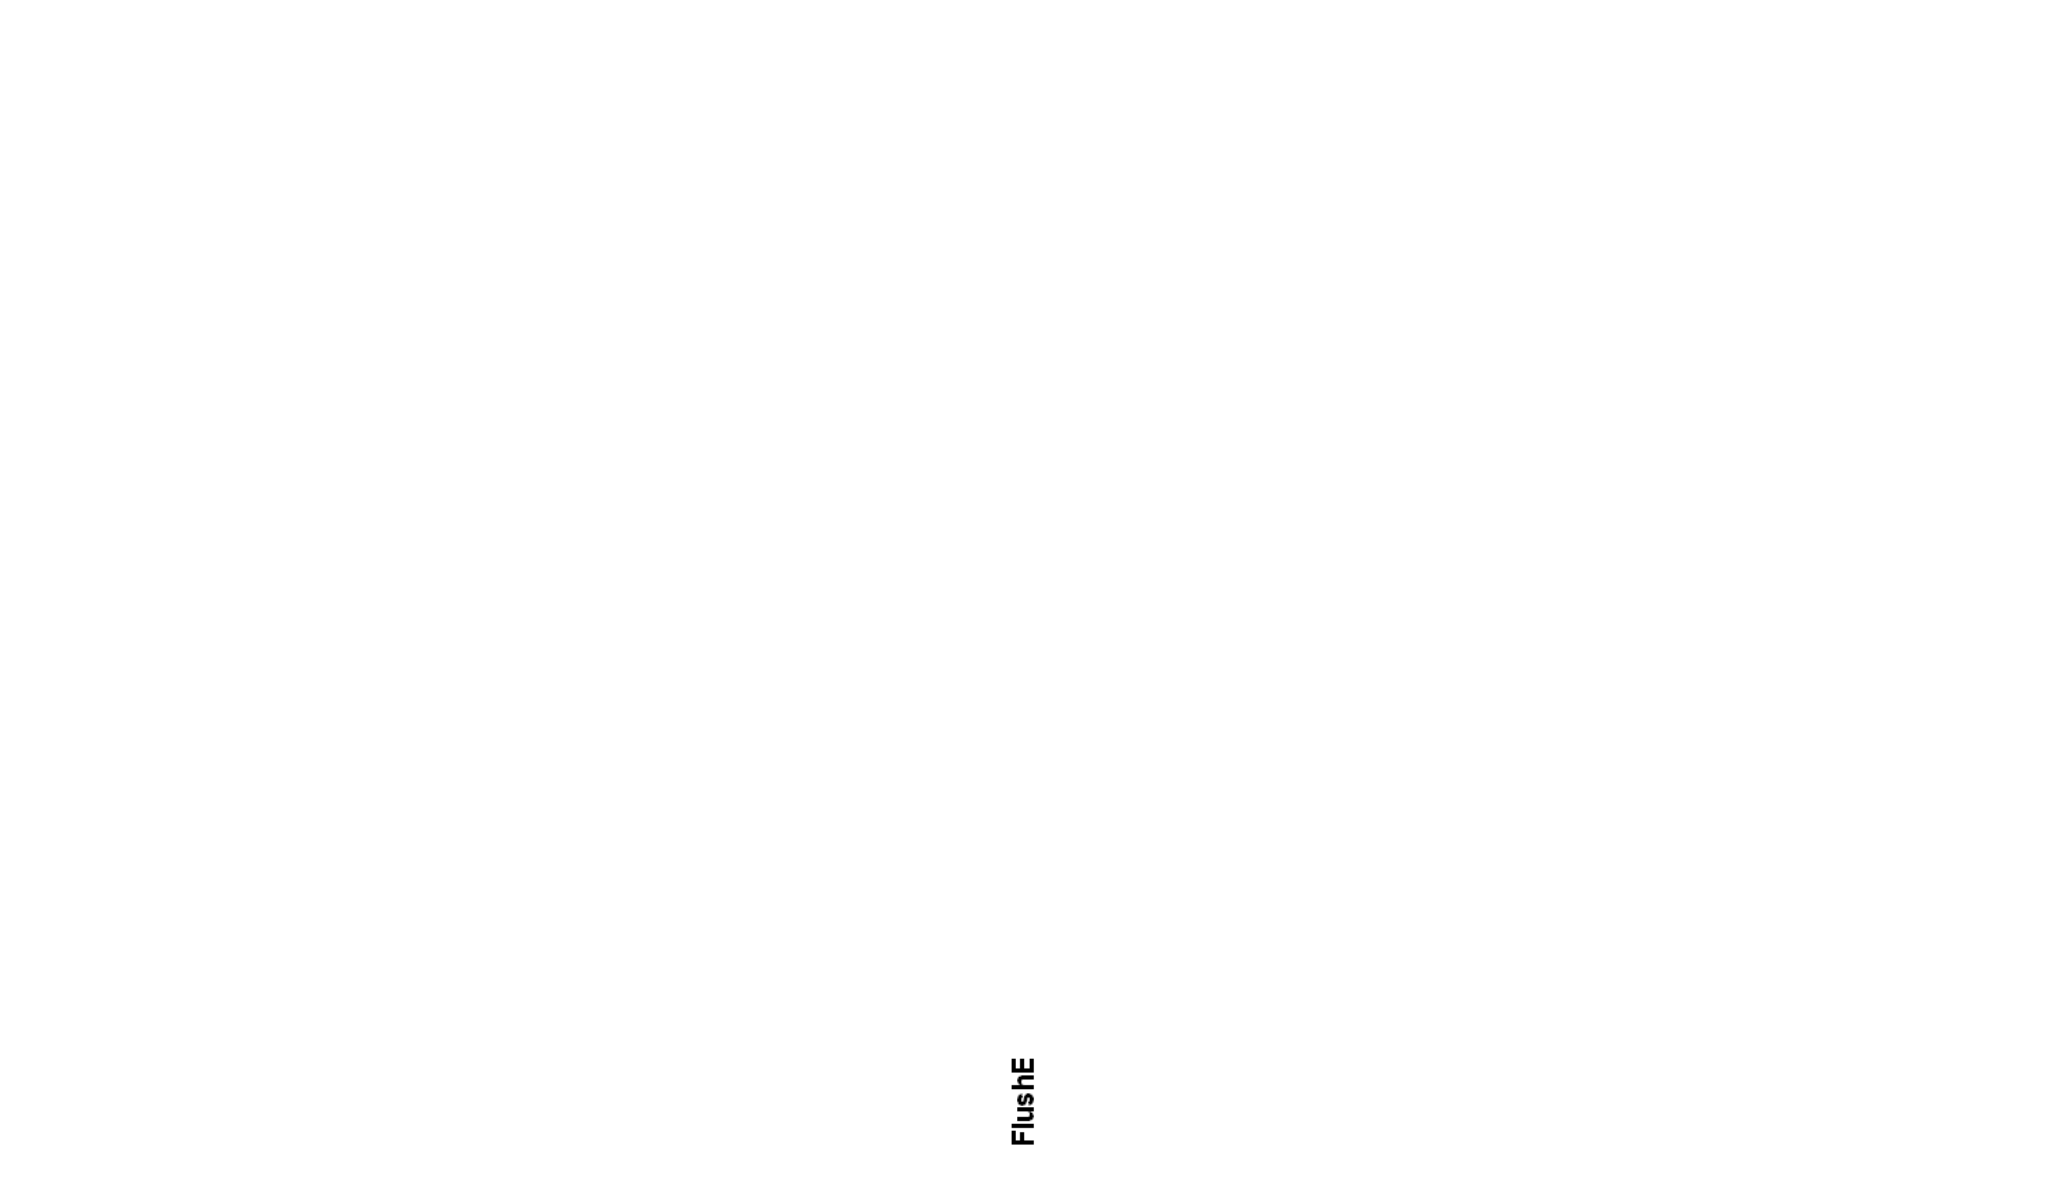
\includegraphics[width=0.9\textwidth]{Qtrvsim-jalr.pdf}
\end{center}

Quiz: How many of the connections are you able to describe their use

\phantom{Quiz: }A -- none B -- about one third  C -- about half D -- almost all.
\end{frame}


\begin{frame}
\frametitle{JALR in QtRvSim Simulator}

\begin{center}
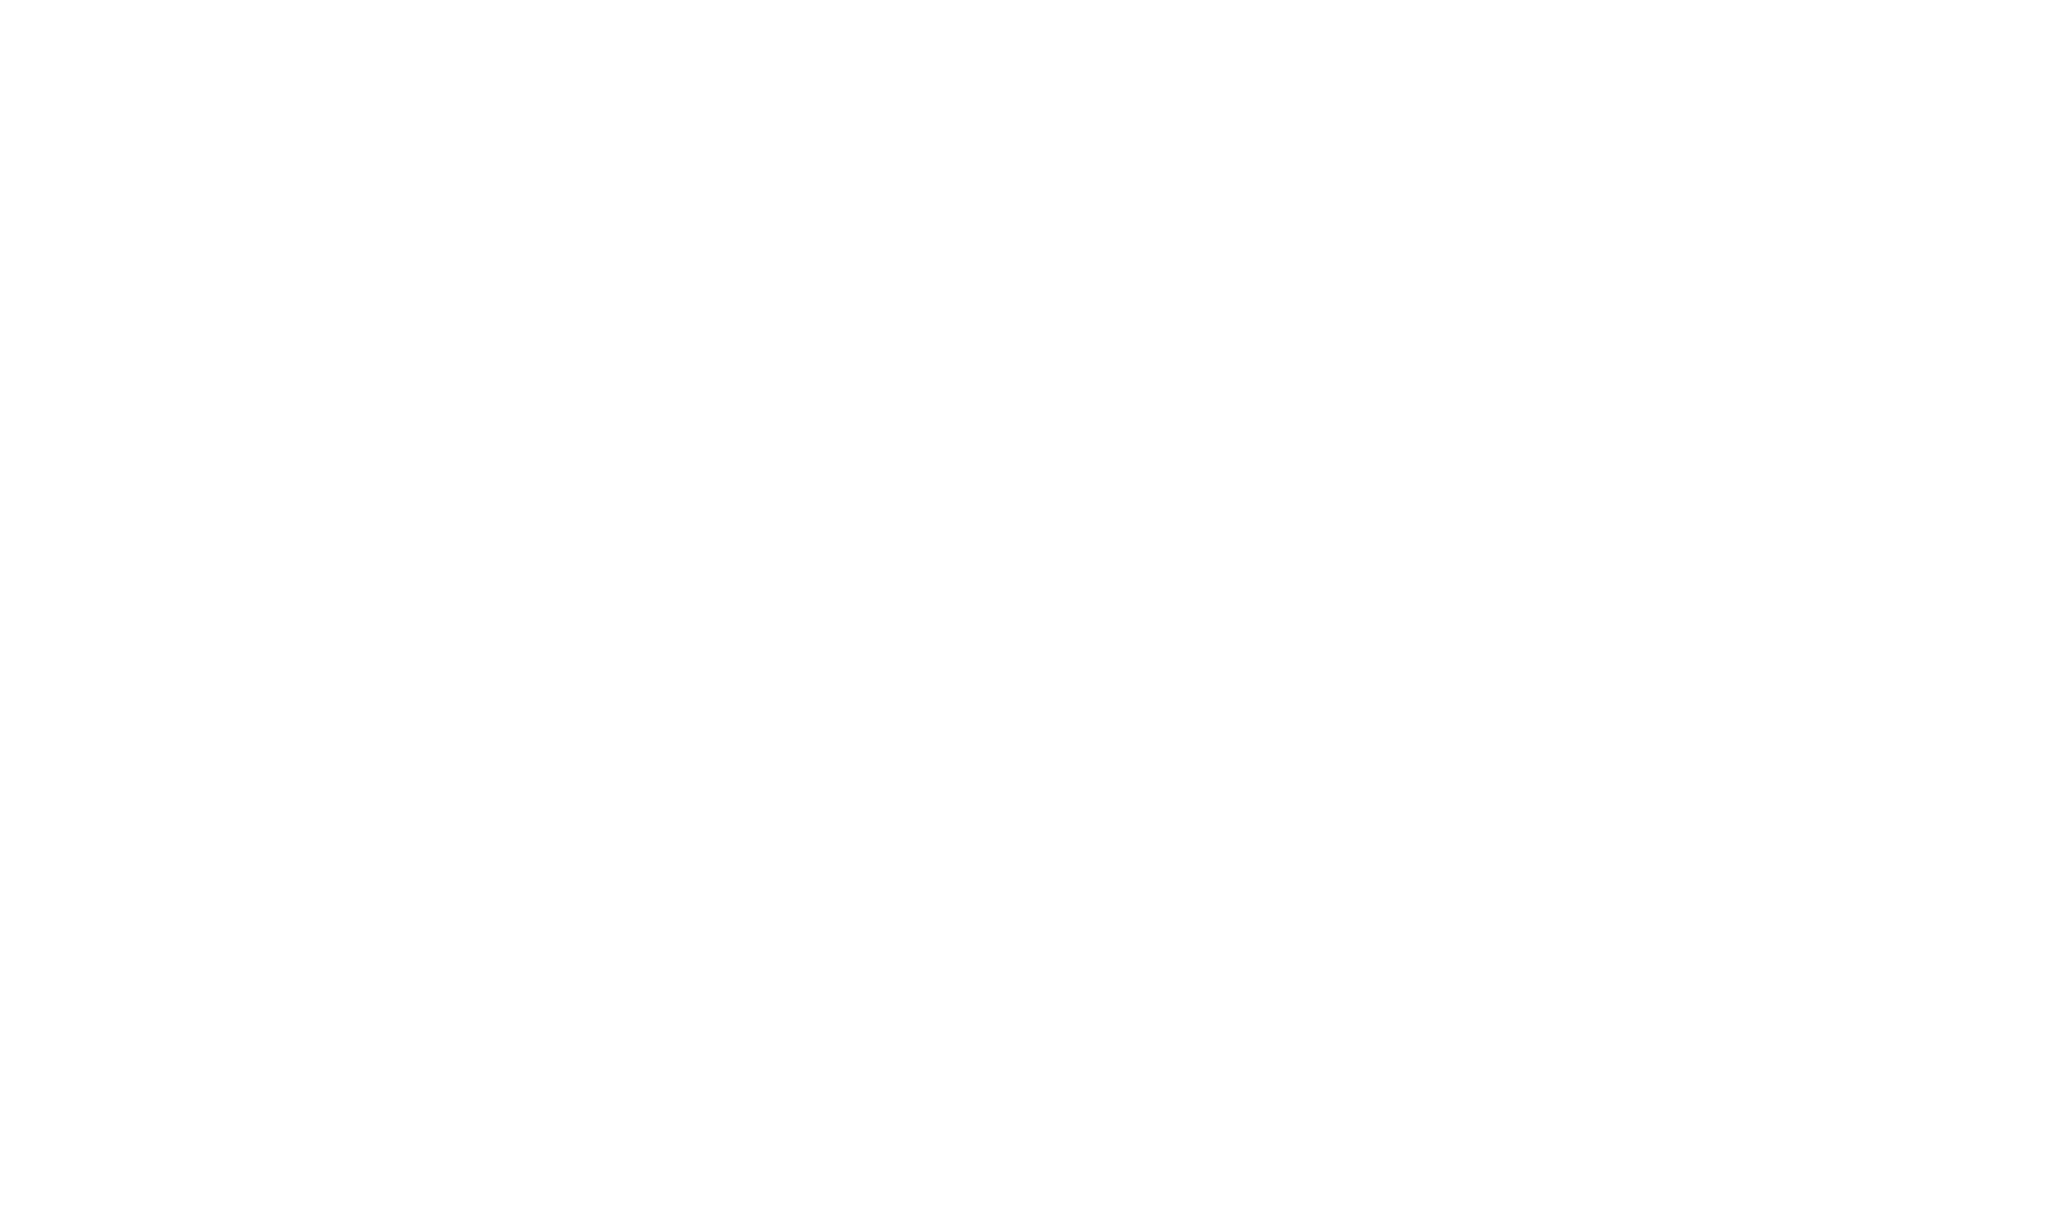
\includegraphics[width=0.9\textwidth]{Jalr-exec.pdf}
\end{center}

\end{frame}



\begin{frame}
\frametitle{JALR -- Control Hazard Caused by Jump}

\begin{center}
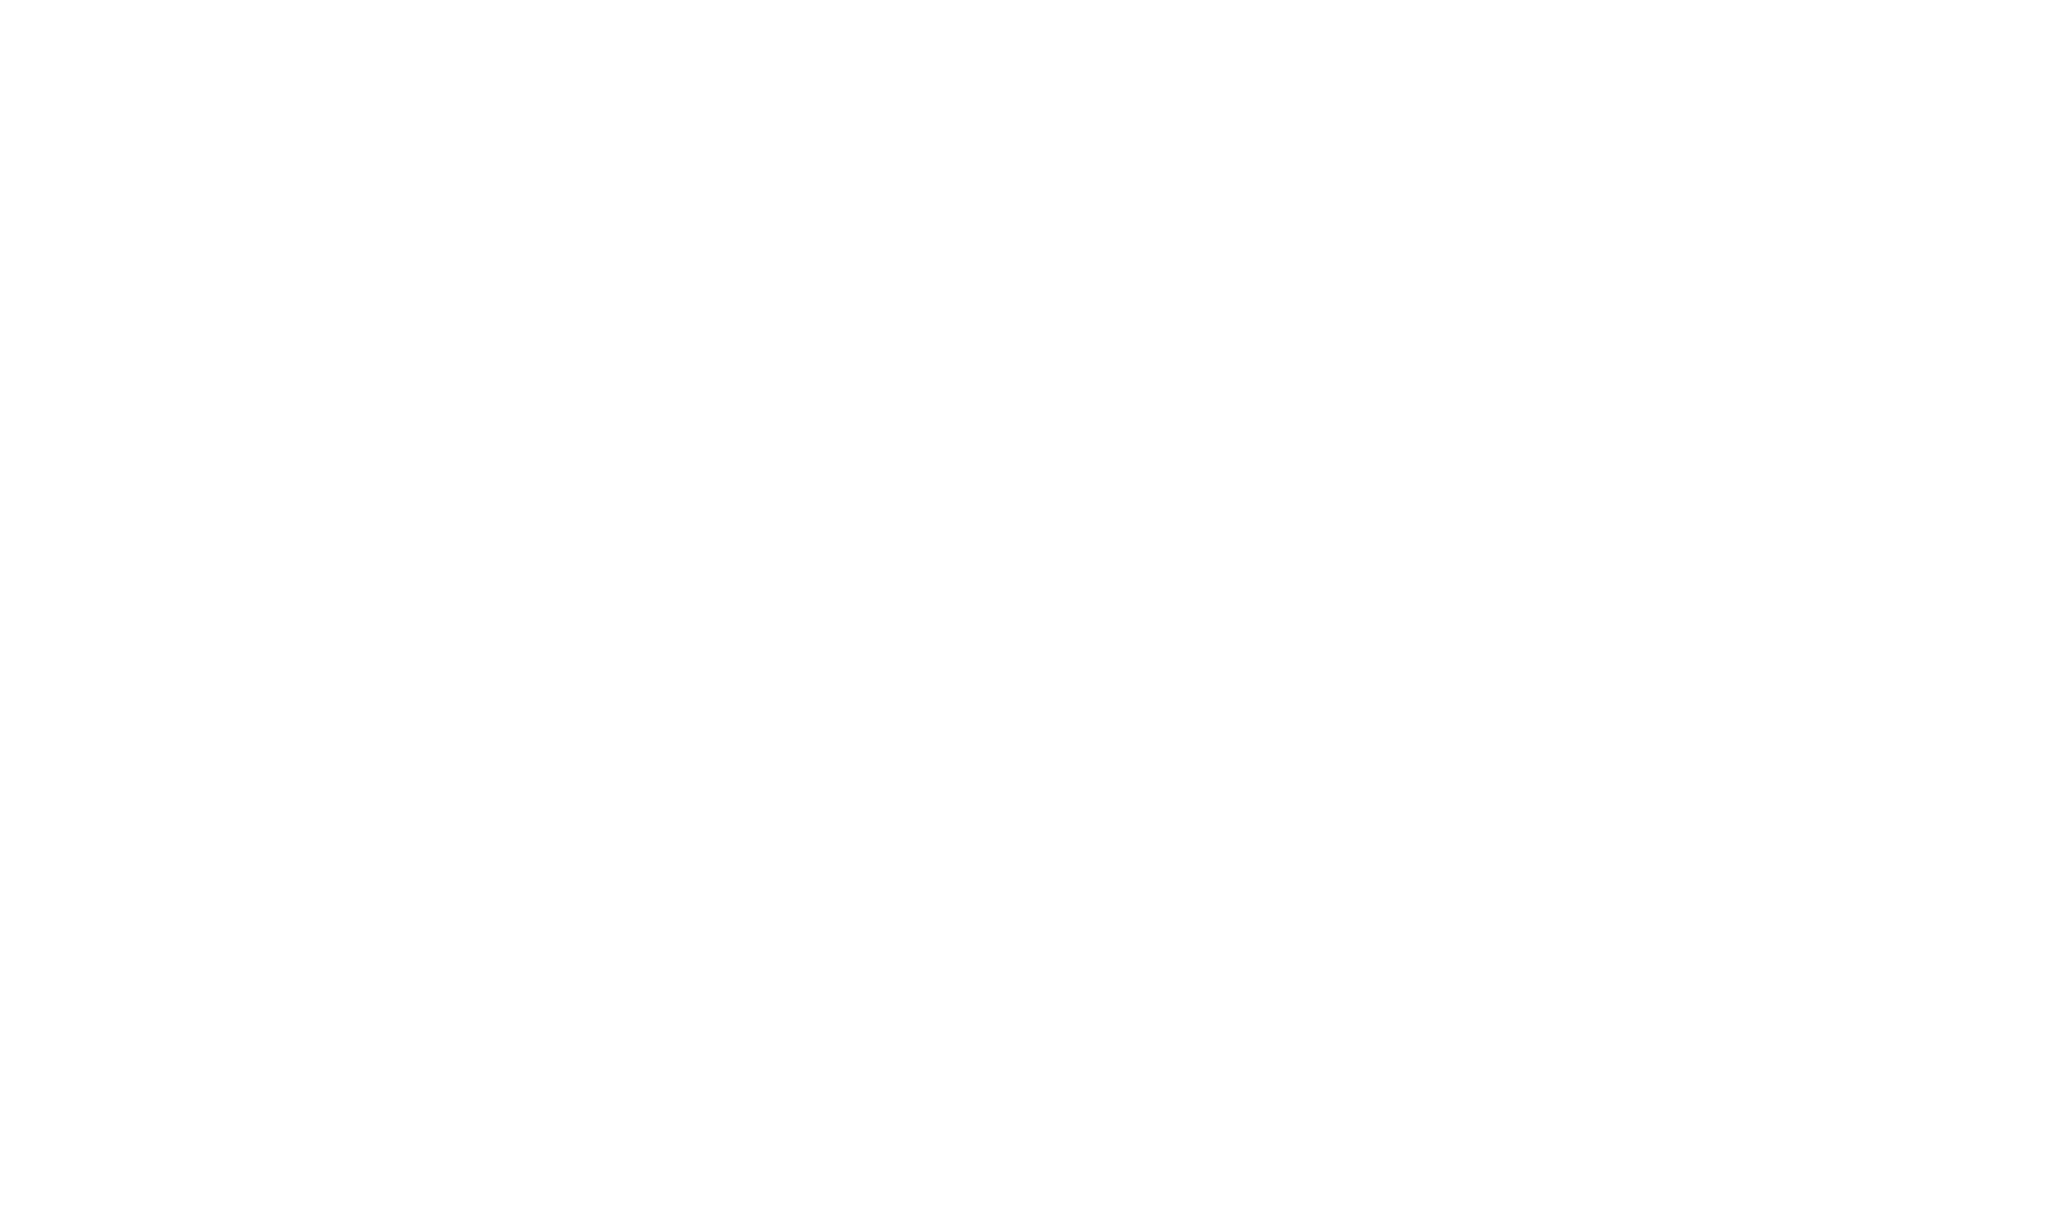
\includegraphics[width=0.9\textwidth]{Jalr-mem.pdf}
\end{center}

\end{frame}



\begin{frame}
\frametitle{What to Do If the Function Calls Another One in Its Body?}

The caller prepares the arguments in registers \texttt{a0} to \texttt{a7} and the return address in register \texttt{ra}.

\bigskip

But how to solve, keep argument values, when a function calls another function in its body?

\bigskip

It is necessary to store the register \texttt{ra} and registers \texttt{a0}--\texttt{a7} somewhere, but where?

\begin{itemize}
\item Activation record or activation frame is used to store function temporary variables over another function call.
\item This record, or frame, is stored on the stack (call stack or stack frame).
\end{itemize}
\end{frame}


\begin{frame}
\frametitle{Stack}

\begin{columns}
\begin{column}{0.7\textwidth}
Stack is LIFO (Last In First Out) data stucture -- the last stored value is retrieved as the fisrt
\begin{itemize}
 \item push -- store data onto stack top, stack is one element deeper
 \item pop -- take value from the top, previous one is on top now
\end{itemize}

Stack implementation where the top is defined by \texttt{sp} (\texttt{x2}) register:
\begin{itemize}
 \item push 
 
\texttt{addi sp, sp, -4 \phantom{xx}}  -- space allocation

\texttt{sw \phantom{xx}x10, 0(sp) \phantom{xx}}  -- value store
 
 \item pop

\texttt{lw \phantom{xx}x10, 0(sp) \phantom{xx}}  -- value restore

\texttt{addi sp, sp, 4 \phantom{xxx}}  -- space release

\end{itemize}

\end{column}
\hfill
\begin{column}{0.3\textwidth}  
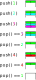
\includegraphics[width=0.9\textwidth]{stack-push-pop.pdf}
\end{column}
\end{columns}

\end{frame}

\begin{frame}
\frametitle{What Is Stored onto Sack in Function?}

Activation or stack frame stores:
\begin{itemize}
 \item Return address and arguments which are used latter when another function is called.
 \item Function local variables, which lifetime is limited by the function body execution.
 \item The ABI specification forbids to return from function with any of \texttt{s0}-\texttt{s11} modified from state at the call
\begin{itemize}
 \item \texttt{s0} register is sometimes used as the pointer to start of an activation frame -- frame \texttt{fp} pointer
 \item \texttt{fp} register points to the fixed stack position during function body and this allows use it in relative addressing of local variables, arguments stored on stack and for final stack restoring if \texttt{alloca} and or dynamic length local arrays are used and allocated by \texttt{sp} register advances.
\end{itemize}
\end{itemize}
\end{frame}


\begin{frame}
\frametitle{RISC-V Calling Convention -- Part of ABI}

Which registers can be freely modified (clobbered) by callee and which registers values have to be preserved to be returned the same to caller.

\begin{tabular}{|c|c|p{4cm}|c|}\hline
Mnemonic & Register & Role in function & Calee \\
   name  &          &       &   can clobber \\ \hline
a0 - a7 & x10 - x17 & function input arguments & yes \\\hline
a0, a1 & x10, x11 & return value/result & yes \\\hline
ra & x1 & return address & no \\\hline
t0 - t6 & x5-7, x28-x31 & temporary/automatic variables & yes \\\hline
s0 - s11 & x8-9, x18-x27 & saved registers & no\\\hline
sp & x2 & stack pointer & no\\\hline
gp & x3 & global (variables) pointer & -- --\\\hline
tp & x4 & thread pointer/thread local store & -- --\\\hline
\end{tabular}
\end{frame}


\begin{frame}
\frametitle{32-bit RISC-V Calling Convetion -- Argument Type Rules}

\begin{itemize}
 \item char, short, int, long, float, pointer -- each argument in single register
 \item long long int, double -- each argument in two registers (the first one aligned to even number)
 \item the content of structure passed by value is copied into as many registers as necessary
 \item if code is compiled for the RISC-V with floting point extension, then fload and double arguments are passed in FPU registers \texttt{f10} -- \texttt{f17}, menmonic designation \texttt{fa0} -- \texttt{fa7}
 \item if the arguments do not fit into appropriate argument registers then the rest is passed on the stack in the new function stack frame prepared for callee
 \item when the function is called (\texttt{jal}/\texttt{jalr} executed), the stack has to be 16 bytes aligned
\end{itemize}
\end{frame}


\begin{frame}
\frametitle{Quiz}

When are some of the registers \texttt{s0}-\texttt{s11} stored onto stack?
\begin{itemize}
 \item[A] never.
 \item[B] when they will be clobbered by calling of another function in the function body.
 \item[C] if they are used for function local variables or \texttt{s0} as \texttt{fp}.
 \item[D] unconditionally each time when function is called.
\end{itemize}
\end{frame}


\begin{frame}
\frametitle{Quiz}

When are some of the registers \texttt{a0}-\texttt{a7} stored onto stack?
\begin{itemize}
 \item[A] never.
 \item[B] if there are so many local variables in the function, that they do not fit into registers.
 \item[C] if the another function is called in the function body and given input argument are used in computation after that call .
 \item[D] only if the function is recurrent (calls itself recursively).
\end{itemize}
\end{frame}


\begin{frame}[fragile]
\frametitle{Function Calling}

\begin{columns}
\begin{column}{0.5\textwidth}
The function calling with max 8 parameters:

\begin{minted}[fontsize=\footnotesize]{c}
t = addfour(1, 2, 3, 4);
\end{minted}

Compiled for RISC-V
\begin{minted}[fontsize=\footnotesize]{gas}
li  a3,4
li  a2,3
li  a1,2
li  a0,1
jal ra,10054 <addfour>
\end{minted}

\end{column}
\begin{column}{0.5\textwidth}  
Calling of the function with 10 arguments:

\begin{minted}[fontsize=\footnotesize]{c}
t = addten(1, 2, 3, 4, 5, 
          6, 7, 8, 9, 10);
\end{minted}

Compiled for RISC-V
\begin{minted}[fontsize=\footnotesize]{gas}
li  a5,10
sw  a5,4(sp)
li  a5,9
sw  a5,0(sp)
li  a7,8
li  a6,7
li  a5,6
li  a4,5
li  a3,4
li  a2,3
li  a1,2
li  a0,1
jal ra,10054 <addten>
\end{minted}
\end{column}
\end{columns}
\end{frame}




\begin{frame}
\frametitle{Function Translation -- Simple Function}

Example with few parameters without internal function call with four local variables
\begin{columns}
\begin{column}{0.65\textwidth}
\begin{itemize}
 \item Space for local/automatic variables is allocated on the stack
 
 \texttt{addi  sp,sp,-16}
 \item Local variables are accessible on the stack:
 
 0(sp), 4(sp), 8(sp), 12(sp)
\begin{itemize}
 \item If there is enough available registers then stack is not for leaf-node function used at all
\end{itemize}
\end{itemize}

Function finalization:
\begin{itemize}
 \item Release/free space for local variables
 
 \texttt{addi  sp,sp,16}
 \item Return to the caller after \texttt{jal}/\texttt{jalr}
 
 \texttt{jalr 0(x1)} -- \texttt{ret} 
\end{itemize}
\end{column}
\begin{column}{0.35\textwidth}  
\includegraphics[width=0.9\textwidth]{simple_fnc-en.pdf}
\end{column}
\end{columns}

\end{frame}


\begin{frame}[fragile,shrink=5]
\frametitle{The Function with 10 Arguments and Call in the Body}

The function allocates space for two local variables in addition.

\begin{columns}
\begin{column}{0.35\textwidth}
Function prologue/start:

\begin{minted}[fontsize=\footnotesize]{gas}
addi  sp,sp,-48
sw  ra,44(sp)
sw  s0,40(sp)
sw  s1,36(sp)
sw  s2,32(sp)
sw  s3,28(sp)
sw  s4,24(sp)
\end{minted}

Access to the local variables:
\begin{minted}[fontsize=\footnotesize]{gas}
lw  t0,8(sp)
lbu t1,15(sp)
\end{minted}

\texttt{int i;} location \texttt{8(sp)}

\texttt{char c;} location \texttt{15(sp)}

\texttt{0(sp)} -- \texttt{7(sp)} unused or reserved for inner call argumens


\end{column}   
\begin{column}{0.29\textwidth}
Function finalization/epilogue:

\begin{minted}[fontsize=\footnotesize]{gas}
lw   ra,44(sp)
lw   s0,40(sp)
lw   s1,36(sp)
lw   s2,32(sp)
lw   s3,28(sp)
lw   s4,24(sp)
addi sp,sp,48
ret
\end{minted}

Remark: the stack allocations are aligned to 16 bytes.

\end{column}
\begin{column}{0.35\textwidth}  
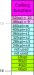
\includegraphics[width=0.7\textwidth]{complex_fnc-en.pdf}
\end{column}
\end{columns}
\end{frame}


\begin{frame}[shrink=5]
\frametitle{Function Frame Pointer}

\begin{itemize}
 \item The function frame pointer contains the value of the \texttt{sp} at function entry
 \item The \texttt{s0} register is used as \texttt{fp} (frame pointer), it is callee save (non-clobberable) register, which has to be saved at function entry and restored at exit.
 \item Advantages of \texttt{fp} use:
\begin{itemize}
 \item Arguments and local variables of the function addressable by fixed offsets to \texttt{fp} even if \texttt{sp} is changed inside function body (e.g. arguments for function calls) which requires offsets to \texttt{sp} recalculations or make it impossible in \texttt{alloca} case
 \item The stack frames unwinding is much easier, i.e. for debugging
\begin{itemize}
 \item Stack unwinding is required even in case of exception processing in C++ when the exception is catch in same function in the caller chain to the throwing function
 \item It is necessary to restore stack into state which corresponds its state inside catching caller function at time of the call of the function leading to the one causing the exception.
\end{itemize}
\end{itemize}
 \item Disadvantages of \texttt{fp} use:
\begin{itemize}
\item Slows down the program, although it is only a few instructions when entering and exiting the function, but if the function is called often and its body is short, it can be a significant overhead.
\item \texttt{fp} occupies the register \texttt{s0}, which could be used to store something else. If there are no free registers, then the value must be stored on the stack in RAM (via cache), which is slower than using the register.
\end{itemize}
\end{itemize}
\end{frame}


\begin{frame}[fragile,shrink=5]
\frametitle{Compile Function with Enforced Frame Pointer}

The GCC compiler switch \texttt{-fno-omit-frame-pointer} is used to enforce frame pointer
\begin{columns}
\begin{column}{0.25\textwidth}
Prologue of the function in RISC-V case

\begin{minted}[fontsize=\footnotesize]{gas}
addi sp,sp,-48
sw   ra,44(sp)
sw   s0,40(sp)
sw   s1,36(sp)
sw   s2,32(sp)
sw   s3,28(sp)
sw   s4,24(sp)
sw   s5,20(sp)
addi s0,sp,48
\end{minted}
\end{column}   
\begin{column}{0.4\textwidth}
Access to the local variable:

\begin{minted}[fontsize=\footnotesize]{gas}
sw a0,-36(s0)
\end{minted}
in the case without \texttt{fp}:
\begin{minted}[fontsize=\footnotesize]{gas}
sw a0, 12(sp)
\end{minted}



Function finalization:

\begin{minted}[fontsize=\footnotesize]{gas}
lw   ra,44(sp)
lw   s0,40(sp)
lw   s1,36(sp)
lw   s2,32(sp)
lw   s3,28(sp)
lw   s4,24(sp)
lw   s5,20(sp)
addi sp,sp,48
ret
\end{minted}
\end{column}
\begin{column}{0.35\textwidth}  
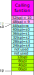
\includegraphics[width=0.7\textwidth]{complex_fnc_fp-en.pdf}
\end{column}
\end{columns}
\end{frame}


\begin{frame}[fragile,shrink=20]
\frametitle{The Homework No. 4 -- Subroutine}

Analyze (reverse engineering source code) of function \texttt{subroutine\_fnc}:
\begin{itemize}
\item find which of \texttt{a0} -- \texttt{a7} are used in function and are filled by arguments before its call
 \begin{itemize}
 \item WARNING: compiler uses \texttt{a\textit{X}} registers as temporal variables for computation same as \texttt{t0} -- \texttt{t6} registers, their values can be changes without care about caller
 \end{itemize}
\item find meaning of return value in \texttt{a0} when \texttt{ret} (\texttt{jalr 0(x1)}) instruction is reached
\item analyze prologue of the function:
 \begin{itemize}
 \item if it starts by instructions sequence similar to
\begin{minted}[fontsize=\footnotesize]{gas}
addi  sp,sp,-48
sw  ra,44(sp)
sw  s0,40(sp)
sw  s1,36(sp)
sw  s2,32(sp)
sw  s3,28(sp)
sw  s4,24(sp)
\end{minted}
\begin{itemize}
 \item then function uses stack to store return address (\texttt{ra}) and local variables or makes \texttt{s\textit{X}} available for local variables
 \item locations \texttt{0(sp)} to \texttt{23(sp)} can be used for local/automatic variables
 \item \texttt{s0} -- \texttt{s4} are used for local variables in this case, usually to keep arguments over other function or system calls
 \end{itemize}
 \item if the function does not contain \texttt{addi sp,sp,-X} then it is a "simple" function which does not use stack
\begin{itemize}
 \item all local/automatic variables and intermediate calculations are stored in unused \texttt{a0} -- \texttt{a7} and \texttt{t0} -- \texttt{t6} registers
 \end{itemize}
 \end{itemize}
 \end{itemize}
\end{frame}


\begin{frame}
\frametitle{Process Address Space Organization -- 32-bit Example}

\begin{columns}
\begin{column}{0.75\textwidth}
Each process has it own memory context with 4GiB of virtual address space:
\small
\begin{itemize}
\item The operating system reserves the top 1GiB for itself (3GiB limit)
\item Stack is below the limit (if the process has multiple threads, then the thread stacks are allocated from heap)
\item Below is space used to map dynamic libraries
\item Dynamically allocated memory grows from global \texttt{.data}+\texttt{.bss} end -- heap (malloc,new/free,delete)
\item Global data (initialized \texttt{.data} and uninitialized \texttt{.bss})
\item Program (.text)
\item Some range above 0 is left unmapped to catch NULL pointer dereference errors.
\end{itemize}
\end{column}   
\begin{column}{0.25\textwidth}  
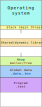
\includegraphics[width=0.8\textwidth]{proc_addr_space-en.pdf}
\end{column}
\end{columns}
\end{frame}

\begin{frame}[fragile,shrink=5]
\frametitle{The Homework No. 4 -- Global Variables}

Global variables presnetce indication:
\begin{itemize}
\item A global variable is a variable defined outside a function, or inside a function using the \texttt{static} keyword
\item Global initialized variables are placed in the \texttt{.data} section, uninitialized (but zeroed in the C case) variables in the \texttt{.bss} section
\item How do I find out if my program has global variables?
\begin{itemize}
\item look at the end of the RISC-V assembler listing and find the \texttt{my\_data} section.

This section might look like this:

\begin{minted}[fontsize=\footnotesize]{gas}
Contents of section my_data:
    11008 00000000                ....
\end{minted}
\begin{itemize}
 \item 11008 is the address in the process virtual address space
 \item 00000000 is hexadecimal listing/representation of the stored data (its initial value)
 \item .... are values displayed as ASCII representation, if the character is unprintable, the dot is on given position
 \item if the global variable/data is used inside code then the access can look as:
\begin{minted}[fontsize=\footnotesize]{gas}
lui  a5, 0x11
addi a5, a5, 8 # 11008
lw   a4, 0(a5)
\end{minted}
 \end{itemize}
 \end{itemize}
 \end{itemize}
\end{frame}


\begin{frame}[fragile]
\frametitle{Quiz}

Consider the function below
\begin{minted}[fontsize=\footnotesize]{c}
int fce (int a) {
  int i;
  
  // function body
  
  return i+a;
}
\end{minted}
Where are argument \texttt{a} and variable \texttt{i} stored in the RISC-V case:
\begin{itemize}
 \item[A] both on the stack or in registers
 \item[B] both in the data section
 \item[C] \texttt{a} on the stack or in register, \texttt{i} in the data section
 \item[D] \texttt{a} in the data section, \texttt{i} on stack or in register
\end{itemize}
\end{frame}


\begin{frame}[fragile,shrink=5]
\frametitle{Security Vulnerability  -- Attacking a Program via the Stack}

\begin{columns}
\begin{column}{0.42\textwidth}
Consider following program:

\begin{minted}[fontsize=\footnotesize]{c}
int virus() {
  // attaceker code
  return 0;
}

int addnumbers(int a, int b, int c, 
  int d, int e, int f, int g, 
  int h, int i, int j) {
  
  volatile int ii,jj=i+j;
  volatile int pole[2];
  
  // some computations
  // function calling
  
  pole[11] = (int)&virus;
  
  return pole[0]+pole[1];
}
\end{minted}
\end{column}   
\begin{column}{0.25\textwidth}
The function prologue:

\begin{minted}[fontsize=\footnotesize]{gas}
addi sp,sp,-48
sw   ra,44(sp)
sw   s0,40(sp)
sw   s1,36(sp)
sw   s2,32(sp)
sw   s3,28(sp)
\end{minted}


\begin{minted}[fontsize=\footnotesize]{gas}
# pole[11]=(int)&virus;
lui  a5,0x10
addi a5,a5,84 # <virus>
sw   a5,44(sp)
\end{minted}

Function epilogue:

\begin{minted}[fontsize=\footnotesize]{gas}
lw   ra,44(sp)
lw   s0,40(sp)
lw   s1,36(sp)
lw   s2,32(sp)
lw   s3,28(sp)
addi sp,sp,48
ret
\end{minted}
\end{column}
\begin{column}{0.33\textwidth}  
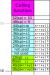
\includegraphics[width=\textwidth]{overflow_fnc-en.pdf}
\end{column}
\end{columns}
\end{frame}



\begin{frame}[fragile]
\frametitle{Variadic Functions in C -- Arguments Access with va\_list}

Definition of the function with variable arguments count:

\begin{columns}
\begin{column}{0.4\textwidth}
\begin{minted}[fontsize=\footnotesize]{c}
#include <stdarg.h>

int sum_n_args(int n, ...) {
  int sum = 0;
  int i;
  va_list ap;
  
  va_start(ap, n);
  for (i=0; i<n; i++) {
    sum+=va_arg(ap,int);
  }
  va_end(ap);
  return sum;
}
\end{minted}
\end{column}   
\begin{column}{0.6\textwidth}
Function calling:

\begin{minted}[fontsize=\footnotesize]{c}
int  main() {
  printf("Sum %d\n", sum_n_args(10, 1,2,3,
                          4,5,6,7,8,9,10);
  printf("Sum %d\n", sum_n_args(2, 1,2);
  printf("Sum %d\n", sum_n_args(8, 1,2,3,
                                4,5,6,7,8);
}
\end{minted}
\end{column}
\end{columns}

\end{frame}

\begin{frame}[fragile,shrink=5]
\frametitle{Translation of the Var. Arg. Function sum\_n\_args}

Preprocessor macros \texttt{va\_start} and \texttt{va\_arg} requires that all arguments are stored in the memory:

\begin{columns}
\begin{column}{0.25\textwidth}
Function prologue:

\begin{minted}[fontsize=\footnotesize]{gas}
addi sp,sp,-64
sw   ra,28(sp)
sw   s0,24(sp)
sw   s1,20(sp)
sw   a1,36(sp)
sw   a2,40(sp)
sw   a3,44(sp)
sw   a4,48(sp)
sw   a5,52(sp)
sw   a6,56(sp)
sw   a7,60(sp)
\end{minted}
\end{column}   
\begin{column}{0.4\textwidth}
\texttt{va\_start(ap, n)}:

\begin{minted}[fontsize=\footnotesize]{gas}
addi a5,sp,36
sw   a5,8(sp)
\end{minted}
\texttt{va\_arg(ap, int)}:
\begin{minted}[fontsize=\footnotesize]{gas}
lw   a4,8(sp)
addi a3,a4,4
sw   a3,8(sp)
lw   s0,0(a4)
\end{minted}

Function epilogue:

\begin{minted}[fontsize=\footnotesize]{gas}
lw   ra,28(sp)
lw   s0,24(sp)
lw   s1,20(sp)
addi sp,sp,64
ret
\end{minted}
\end{column}
\begin{column}{0.3\textwidth}  
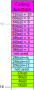
\includegraphics[width=0.7\textwidth]{vaarg_fnc_fp-en.pdf}
\end{column}
\end{columns}
\end{frame}


\section {Operating System Services -- System Calls}

\begin{frame}
\frametitle{Basic of Operating System Protection Mechanisms}

\begin{itemize}
\item A user process cannot directly access the computer's HW.
\item A user process must ask the OS to make the HW available or to handle a request.
\item OS offers services with HW privileged access to processes in form of system calls.
\item Unlike a function call, we do not know the addresses of functions in the kernel.
\item A system call function is selected by the system call number.
\item The actual function call is realized through an interrupt or exception with a specialized instruction:
\begin{itemize}
\item x86 old -- uses int 0x80 directly -- invoke interrupt number 0x80.
\item x86 newer -- specialized instructions sysenter/syscall -- direct, no interrupt gates and accesses less memory $\rightarrow$ is faster.
\item RISC-V -- specialized instruction ecall -- invokes exception.
\end{itemize}
\item Interrupt/exception is handled by the service routine starting at preconfigured address (i.e. \texttt{mtvec}/\texttt{stvec}) in priviledged mode (system or machine) and the user cannot change it.

\end{itemize}
\end{frame}

\begin{frame}
\frametitle{Device Input Realized by System Calls}

The user program prepares the call parameters and system call number in the registers and triggers a special interrupt/exception (\texttt{ecall} on RISC-V).

The OS calls the corresponding function based on the system call number.

\begin{center}
  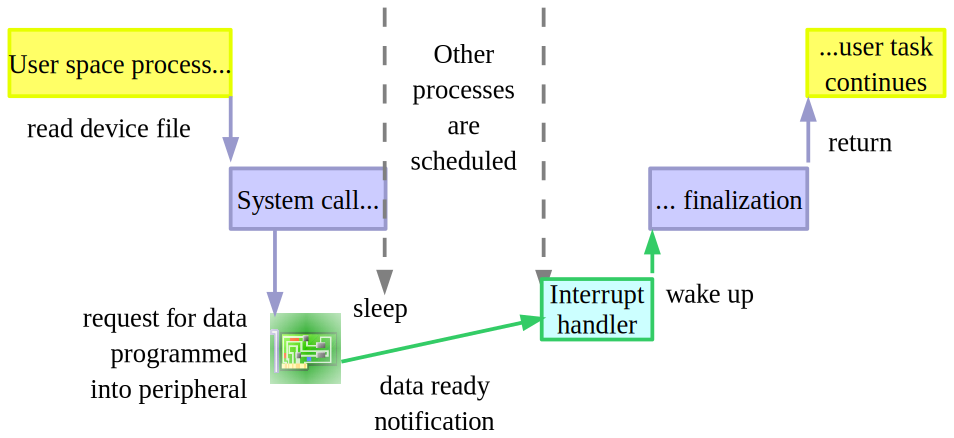
\includegraphics[width=0.95\textwidth]{irq-and-os-en.pdf}
\end{center}

Return from system call to user program uses same or similar mechanism as return
from interrupt/exception (usually \texttt{sret} on RISC-V).
\end{frame}

\begin{frame}[shrink=5]
\frametitle{Application Binary Interface (ABI) -- System Calls}

\begin{itemize}
\item API -- application programming interface -- standard, which function can program call program from libraries.
\begin{itemize}
\item API is defined for the C language by header files.
\item API also defines what the given functions do, what are their return values, how they behave in error case
\item try e.g. \texttt{man 2 read}
\end{itemize}
\item ABI -- application binary interface -- description of which registers and which instructions to use
\item ABI for system calls on the RISC-V architecture
\begin{itemize}
\item \texttt{a7} -- contains the system call number (for an overview, e.g. \url{https://jborza.com/post/2021-05-11-riscv-linux-syscalls/} or \url{https://marcin.juszkiewicz.com.pl/download/tables/syscalls.html})
\item \texttt{a0} to \texttt{a5} -- system call parameters (Linux system calls have a maximum of 6 parameters)
\item a system call is made with the \texttt{ecall} instruction
\item \texttt{a0} contains the return value of the system call
\begin{itemize}
\item if the call should return more data (e.g. reading from a file), the user must specify a pointer to the buffer and the size of the buffer where the OS will write the data.
\end{itemize}
\end{itemize}
\end{itemize}

\end{frame}

\begin{frame}[fragile]
\frametitle{Hello World! Example for RISC-V and Linux kernel}


\begin{minted}[fontsize=\footnotesize]{gas}
.global _start
.text
_start:
#   write(1, "Hello world!\n", 13);
   addi  a7, zero, 64
   addi  a0, zero, 1
   la    a1, zero, text_1
   addi  a2, zero, 13
   ecall
final:
#   exit(0);
   addi  a7, zero, 93
   addi  a0, zero, 0
   ecall
   ebreak
   j final
.data
# store ASCII text, no termination
text_1: .ascii "Hello world!\n"
\end{minted}
\end{frame}


\begin{frame}[fragile]
\frametitle{The Homework No. 4 -- System Calls}

How to identify and analyze system calls?
\begin{itemize}
\item locate \texttt{ecall} instructions.
\item determine value set in \texttt{a7} before \texttt{ecall}, it specifies which system service is requested.
\item find out the values ​​of registers \texttt{a0}, \texttt{a1}, \texttt{a2} (or \texttt{a3} if used).
\item find out corresponding function prototype in the C runtime library and combine it with found arguments.
\item Example: you find out that register \texttt{a7} has the value 63 -- \texttt{read}, re-implement code as the system library function call
\begin{minted}[fontsize=\footnotesize]{c}
read(a0, a1, a2);
\end{minted}
\begin{itemize}
\item the only problem is with the function \texttt{open}/\texttt{openat}, whose \texttt{O\_\textit{XXXX}} flags have different values ​​for the x86 system and for RISC-V
\item because programs are checked by Brute on the x86 system, it is better to verify the values ​​of the parameters in the dump program-x86.list
 \end{itemize}
\end{itemize}
\end{frame}

\begin{frame}
\frametitle{x86 Linux Kernel System Calls}

\begin{itemize}
\item the system call is realized by the instruction \texttt{int 0x80}.
\item the system call number is passed in the \texttt{eax} register.
\begin{itemize}
\item ATTENTION the x86 and RISC-V system call numbers are different.
\end{itemize}
\item system call parameters are stored sequentially in registers:
\begin{itemize}
\item ebx
\item ecx
\item edx
\item esi
\item edi
\item ebp
\end{itemize}
\item In the next lecture, x86 assembler will be described which allows to use x86 code variant listing to be used to solve homework 4.
\end{itemize}
\end{frame}


\begin{frame}[fragile]
\frametitle{Quiz}

Consider the function bellow
\begin{minted}[fontsize=\footnotesize]{c}
int fce (int a) {
  static int s;
  int i;
  
  // telo funkce
  
  return i+s;
}
\end{minted}
Where are variables \texttt{s} and \texttt{i} located?
\begin{itemize}
 \item[A] both allocated on the stack
 \item[B] both in the \texttt{.data} section
 \item[C] \texttt{s} on the stack, \texttt{i} in the \texttt{.data} section
 \item[D] \texttt{s} in the \texttt{.data} section, \texttt{i} on the stack
\end{itemize}
\end{frame}


\end{document}

